\section{Техническое задание}
\subsection{Основание для разработки}

Основанием для разработки является задание на курсовую работу "<Разработка web-сайта \textquotedbl Портфолио фотографа\textquotedbl\".

\subsection{Цель и назначение разработки}

Основной задачей выпускной квалификационной работы является 
разработка сайта-портфолио фотографа.

Задачами данной разработки являются:
\begin{itemize}
\item создание раздела сайта с фотографиями.;
\item реализация формы для добавления фотографий.;
\end{itemize}

\subsection{Требования пользователя к интерфейсу web-сайта}

Сайт должен включать в себя:
\begin{itemize}
    \item навигацию по фотографиям.;
    \item авторизацию в административную панель.;
    \item доступы для администратора, пользователя.;
    \item возможность добавления фотографий.;
\end{itemize}

Композиция шаблона сайта представлена на рисунке ~\ref{maket:image}.

\begin{figure}[ht]
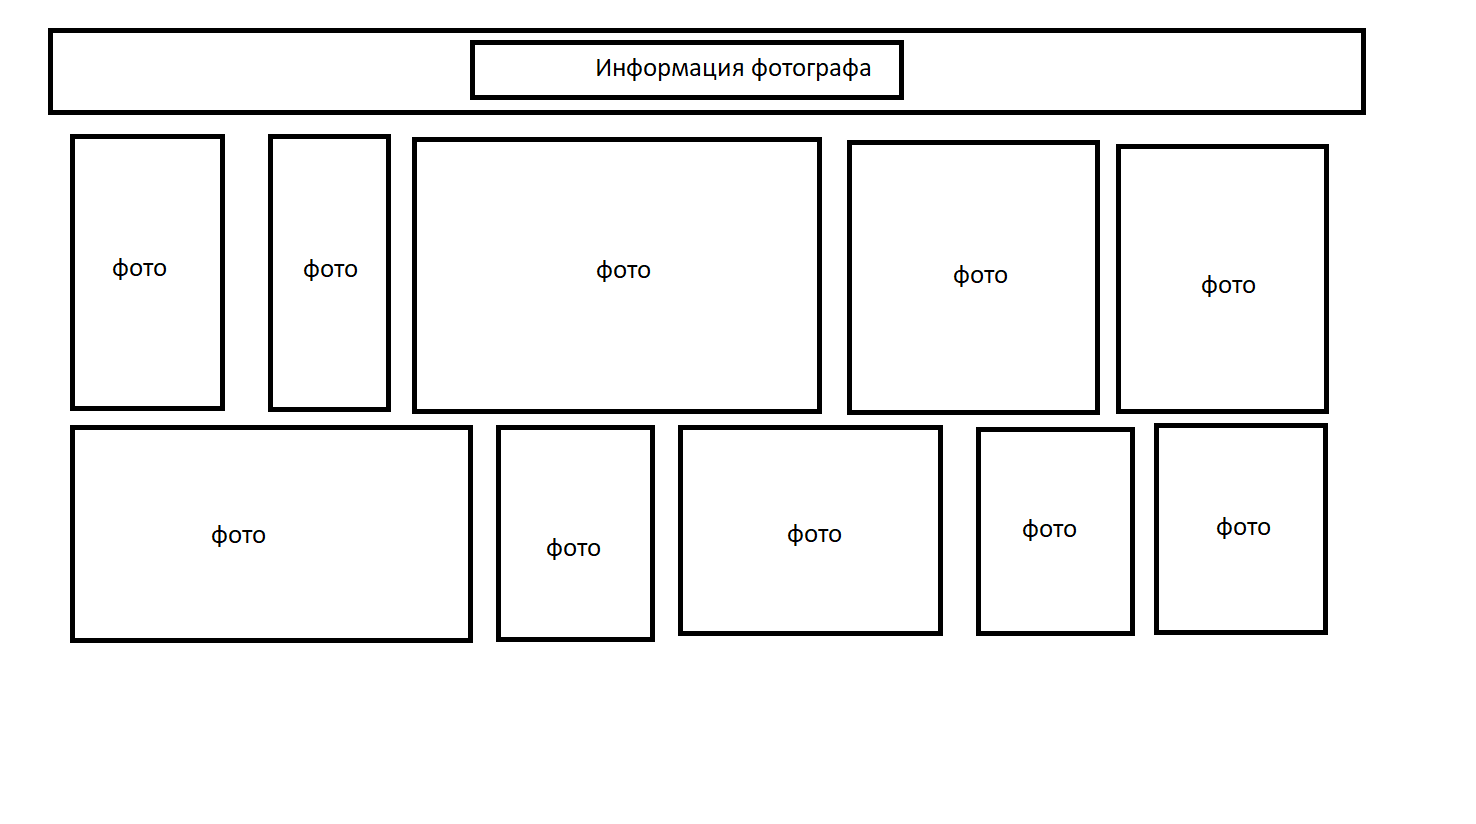
\includegraphics[width=1\linewidth]{плакат1.png}
\caption{Композиция шаблона сайта}
\label{maket:image}
\end{figure}
%\vspace{-\figureaboveskip} % двойной отступ не нужен (можно использовать, если раздел заканчивается картинкой)

\subsection{Моделирование вариантов использования}

Для разрабатываемого сайта была реализована модель, которая обеспечивает наглядное представление вариантов использования сайта.

Она помогает в физической разработке и детальном анализе взаимосвязей объектов. При построении диаграммы вариантов использования применяется унифицированный язык визуального моделирования UML.

Диаграмма вариантов описывает функциональное назначение разрабатываемой системы. То есть это то, что система будет непосредственно делать в процессе своего функционирования. Она является исходным концептуальным представлением системы в процессе ее проектирования и разработки. Проектируемая система представляется в виде ряда прецедентов, предоставляемых системой актерам или сущностям, которые взаимодействуют с системой. Актером или действующим лицом является сущность, взаимодействующая с системой извне (например, человек, техническое устройство). Прецедент служит для описания набора действий, которые система предоставляет актеру.

На основании анализа предметной области в программе должны быть реализованы следующие прецеденты:
\begin{enumerate}
\item Авторизация администратора.
\item Просмотр фотографий.
\item Добавление фотографий.
\end{enumerate}

\subsection{Требования к оформлению документации}

Разработка программной документации и программного изделия должна производиться согласно ГОСТ 19.102-77 и ГОСТ 34.601-90. Единая система программной документации.
